% !TEX program = lualatex
\documentclass[aspectratio=169]{beamer}
\usepackage[utf8]{inputenc}
\usepackage[T1]{fontenc}
\usepackage{graphicx}
\usepackage{hyperref}
\usepackage{xcolor}
\usepackage{listings}
\usepackage{tikz}
\usepackage{fontawesome}
\usepackage{multicol}
\usepackage{booktabs}

% Theme customization
\usetheme{Madrid}
\usecolortheme{default}
\setbeamertemplate{navigation symbols}{}
\setbeamertemplate{footline}[frame number]
\setbeamertemplate{itemize items}[square]
\setbeamertemplate{enumerate items}[default]

% Colors
\definecolor{githubblue}{RGB}{36, 41, 46}
\definecolor{githubgreen}{RGB}{40, 167, 69}
\definecolor{githuborange}{RGB}{240, 140, 45}
\definecolor{githubred}{RGB}{215, 58, 73}
\definecolor{githubgray}{RGB}{88, 96, 105}
\definecolor{codebg}{RGB}{246, 248, 250}

% Title page colors
\setbeamercolor{title}{fg=white}
\setbeamercolor{subtitle}{fg=white}
\setbeamercolor{author}{fg=white}
\setbeamercolor{date}{fg=white}
\setbeamercolor{frametitle}{fg=white,bg=githubblue}

% CRITICAL FIX: Escape # properly for LuaLaTeX
\makeatletter
\lst@CCPutMacro
\lst@ProcessOther {"23}{%
	\lst@ttfamily
	{\raisebox{0.2ex}{\tiny\#}}%
	{\raisebox{0.2ex}{\tiny\#}}}%
\@empty\z@\@empty
\makeatother

% Code listing style
\lstset{
	basicstyle=\ttfamily\small,
	backgroundcolor=\color{codebg},
	breaklines=true,
	breakatwhitespace=false,
	frame=single,
	framesep=3pt,
	rulecolor=\color{githubgray},
	keywordstyle=\color{githubblue}\bfseries,
	commentstyle=\color{githubgreen}\itshape,
	stringstyle=\color{githuborange},
	showstringspaces=false,
	tabsize=2,
	captionpos=b,
	escapeinside={(*@}{@*)},
}

\title{\textbf{Mastering Git \& GitHub}}
\subtitle{A Comprehensive Guide to Version Control}
\author{Your Name}
\date{\today}
\institute{Your Organization}

\begin{document}
	
	% ============ TITLE SLIDE ============
	\begin{frame}[plain]
		\begin{tikzpicture}[remember picture,overlay]
			\fill[githubblue] (current page.south west) rectangle (current page.north east);
			\node[white] at (current page.center) {
				\begin{minipage}{0.8\textwidth}
					\centering
					{\Huge\bfseries Mastering Git \& GitHub}\\[0.5cm]
					{\Large A Comprehensive Guide to Version Control}\\[1cm]
					{\large Your Name}\\[0.3cm]
					{\small \today}\\[0.3cm]
					{\small Your Organization}
				\end{minipage}
			};
		\end{tikzpicture}
	\end{frame}
	
	% ============ OUTLINE ============
	\begin{frame}{Table of Contents}
		\tableofcontents[hideallsubsections]
	\end{frame}
	
	% ============ SECTION 1: INTRODUCTION ============
	\section{Introduction to Version Control}
	
	\begin{frame}{What is Version Control?}
		\begin{columns}
			\column{0.5\textwidth}
			\begin{block}{Definition}
				Version control is a system that records changes to a file or set of files over time so that you can recall specific versions later.
			\end{block}
			\begin{itemize}
				\item Track every modification
				\item Revert files or entire project to previous state
				\item Compare changes over time
				\item See who last modified something
			\end{itemize}
			
			\column{0.5\textwidth}
			\begin{center}
				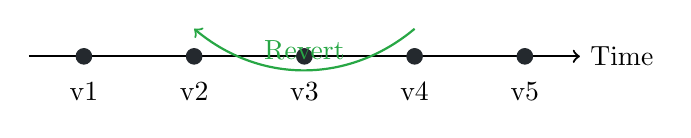
\begin{tikzpicture}[scale=0.7]
					\draw[thick, ->] (0,0) -- (10,0) node[right] {Time};
					\foreach \x/\label in {1/v1,3/v2,5/v3,7/v4,9/v5} {
						\filldraw[githubblue] (\x,0) circle (4pt);
						\node[below] at (\x,-0.3) {\label};
					}
					\draw[githubgreen, thick, ->, bend left=40] (7,0.5) to node[above] {Revert} (3,0.5);
				\end{tikzpicture}
				\vspace{0.5cm}
				\textit{Version control timeline visualization}
			\end{center}
		\end{columns}
	\end{frame}
	
	\begin{frame}{Why Use Version Control?}
		\begin{multicols}{2}
			\begin{itemize}
				\item \textbf{Collaboration}
				\begin{itemize}
					\item Multiple developers work simultaneously
					\item No file conflicts or overwrites
				\end{itemize}
				\vspace{0.3cm}
				\item \textbf{Backup \& Restore}
				\begin{itemize}
					\item Complete history preserved
					\item Revert to any previous state
				\end{itemize}
				\vspace{0.3cm}
				\item \textbf{Tracking Changes}
				\begin{itemize}
					\item Who made what changes
					\item When and why changes were made
				\end{itemize}
			\end{itemize}
			
			\columnbreak
			
			\begin{itemize}
				\item \textbf{Branching \& Merging}
				\begin{itemize}
					\item Experiment safely
					\item Feature isolation
				\end{itemize}
				\vspace{0.3cm}
				\item \textbf{Code Review}
				\begin{itemize}
					\item Quality assurance
					\item Knowledge sharing
				\end{itemize}
				\vspace{0.3cm}
				\item \textbf{Continuous Integration}
				\begin{itemize}
					\item Automated testing
					\item Automated deployment
				\end{itemize}
			\end{itemize}
		\end{multicols}
	\end{frame}
	
	\begin{frame}{Types of Version Control Systems}
		\begin{columns}[T]
			\column{0.5\textwidth}
			\begin{block}{Centralized (CVCS)}
				\begin{itemize}
					\item Single central server
					\item Examples: SVN, CVS
					\item \textcolor{red}{Single point of failure}
					\item \textcolor{red}{Network dependency}
				\end{itemize}
			\end{block}
			
			\column{0.5\textwidth}
			\begin{block}{Distributed (DVCS)}
				\begin{itemize}
					\item Every user has full repository
					\item Examples: Git, Mercurial
					\item \textcolor{green}{Work offline}
					\item \textcolor{green}{No single point of failure}
				\end{itemize}
			\end{block}
		\end{columns}
		
		\vspace{0.5cm}
		\begin{center}
			\textbf{Git is the world's most popular DVCS}
		\end{center}
	\end{frame}
	
	% ============ SECTION 2: GIT FUNDAMENTALS ============
	\section{Git Fundamentals}
	
	\begin{frame}{What is Git?}
		\begin{columns}
			\column{0.6\textwidth}
			\begin{itemize}
				\item Created by Linus Torvalds in 2005
				\item Free and open source
				\item Designed for speed and efficiency
				\item Strong support for non-linear development
				\item Fully distributed
				\item Handles large projects efficiently
			\end{itemize}
			
			\column{0.4\textwidth}
			\begin{center}
				
\begin{tikzpicture}
					\node[circle, fill=githuborange, minimum size=3cm, text=white] {
						\begin{tabular}{c}
							\Huge \textbf{Git}\\
							\small Distributed VCS
						\end{tabular}
					};
				\end{tikzpicture}
			\end{center}
		\end{columns}
	\end{frame}
	
	\begin{frame}{Git Installation}
		\begin{alertblock}{Installation Methods}
			\begin{description}
				\item[Windows] Download from \href{https://git-scm.com}{git-scm.com} or use \texttt{winget install Git.Git}
				\item[macOS] \texttt{brew install git} (Homebrew) or Xcode Command Line Tools
				\item[Linux (Ubuntu/Debian)] \texttt{sudo apt-get install git}
				\item[Linux (Fedora)] \texttt{sudo dnf install git}
			\end{description}
		\end{alertblock}
		
		\vspace{0.3cm}
		\begin{exampleblock}{Verify Installation}
			\texttt{\$ git --version}
		\end{exampleblock}
	\end{frame}
	
	\begin{frame}[fragile]{Git Configuration}
		\begin{block}{Essential Configuration}
			\begin{lstlisting}[language=bash]
				# Set your identity
				git config --global user.name "Your Name"
				git config --global user.email "your.email@example.com"
				
				# Set default branch name
				git config --global init.defaultBranch main
				
				# Set default editor
				git config --global core.editor "code --wait"
				
				# View all configurations
				git config --list
			\end{lstlisting}
		\end{block}
		
		\begin{itemize}
			\item \texttt{--global}: Applies to all repositories for current user
			\item \texttt{--local}: Applies to current repository only (default)
			\item \texttt{--system}: Applies to all users on the system
		\end{itemize}
	\end{frame}
	
	\begin{frame}{Git Three States}
		\begin{center}
			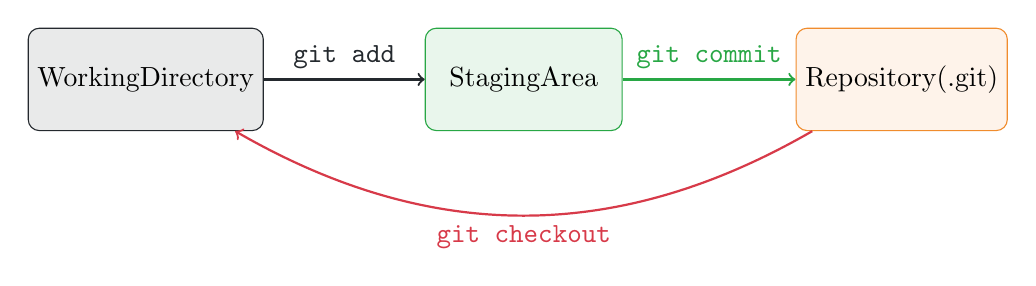
\begin{tikzpicture}[node distance=3cm, auto, scale=0.9]
				\node[rectangle, draw=githubblue, fill=githubblue!10, minimum width=2.5cm, minimum height=1.3cm, rounded corners] (wd) {Working\\Directory};
				\node[rectangle, draw=githubgreen, fill=githubgreen!10, minimum width=2.5cm, minimum height=1.3cm, rounded corners, right of=wd, xshift=1.8cm] (sa) {Staging\\Area};
				\node[rectangle, draw=githuborange, fill=githuborange!10, minimum width=2.5cm, minimum height=1.3cm, rounded corners, right of=sa, xshift=1.8cm] (repo) {Repository\\(.git)};
				
				\draw[->, thick, githubblue] (wd) -- node[above] {\texttt{git add}} (sa);
				\draw[->, thick, githubgreen] (sa) -- node[above] {\texttt{git commit}} (repo);
				\draw[->, thick, githubred, bend left=30] (repo) to node[below] {\texttt{git checkout}} (wd);
			\end{tikzpicture}
		\end{center}
		
		\vspace{0.3cm}
		\begin{description}
			\item[Working Directory] Where you modify files
			\item[Staging Area] Files marked for next commit
			\item[Repository] Committed history stored in \texttt{.git}
		\end{description}
	\end{frame}
	
	\begin{frame}[fragile]{Basic Git Commands}
		\begin{columns}[T]
			\column{0.5\textwidth}
			\begin{block}{Repository Operations}
				\begin{lstlisting}[language=bash]
					# Initialize repository
					git init
					
					# Clone repository
					git clone <url>
					
					# Check status
					git status
					
					# Add files to staging
					git add <file>
					git add .  # Add all
					
					# Commit changes
					git commit -m "message"
					
					# View history
					git log
					git log --oneline --graph
				\end{lstlisting}
			\end{block}
			
			\column{0.5\textwidth}
			\begin{block}{Working with Changes}
				\begin{lstlisting}[language=bash]
					# View differences
					git diff
					git diff --staged
					
					# Remove files
					git rm <file>
					git rm --cached <file>
					
					# Move/rename files
					git mv <old> <new>
					
					# Undo changes
					git restore <file>
					git restore --staged <file>
					
					# Amend last commit
					git commit --amend
				\end{lstlisting}
			\end{block}
		\end{columns}
	\end{frame}
	
	% ============ SECTION 3: BRANCHING & MERGING ============
	\section{Branching \& Merging}
	
	\begin{frame}{Understanding Branches}
		\begin{columns}
			\column{0.5\textwidth}
			\begin{itemize}
				\item A branch is a movable pointer to a commit
				\item Default branch is usually \texttt{main} or \texttt{master}
				\item Branches allow parallel development
				\item Lightweight and fast to create
				\item Essential for feature development
			\end{itemize}
			
			\column{0.5\textwidth}
			\begin{center}
				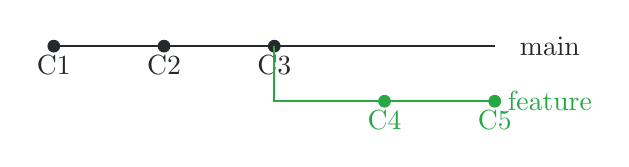
\begin{tikzpicture}[scale=0.7]
					\draw[thick, githubblue] (0,2) -- (8,2);
					\node[githubblue] at (9,2) {main};
					\filldraw[githubblue] (0,2) circle (3pt) node[below] {C1};
					\filldraw[githubblue] (2,2) circle (3pt) node[below] {C2};
					\filldraw[githubblue] (4,2) circle (3pt) node[below] {C3};
					
					\draw[thick, githubgreen] (4,2) -- (4,1) -- (8,1);
					\node[githubgreen] at (9,1) {feature};
					\filldraw[githubgreen] (6,1) circle (3pt) node[below] {C4};
					\filldraw[githubgreen] (8,1) circle (3pt) node[below] {C5};
				\end{tikzpicture}
			\end{center}
		\end{columns}
	\end{frame}
	
	\begin{frame}[fragile]{Branch Commands}
		\begin{block}{Branch Management}
			\begin{lstlisting}[language=bash]
				# List branches
				git branch
				git branch -a  # Include remote branches
				
				# Create branch
				git branch <branch-name>
				
				# Switch to branch
				git checkout <branch-name>
				# OR (Git 2.23+)
				git switch <branch-name>
				
				# Create and switch
				git checkout -b <branch-name>
				git switch -c <branch-name>
				
				# Delete branch
				git branch -d <branch-name>
				git branch -D <branch-name>  # Force delete
				
				# Rename branch
				git branch -m <old-name> <new-name>
			\end{lstlisting}
		\end{block}
	\end{frame}
	
	\begin{frame}{Merging Strategies}
		\begin{columns}[T]
			\column{0.5\textwidth}
			\begin{block}{Fast-Forward Merge}
				\begin{itemize}
					\item No divergent work
					\item Simply moves pointer forward
					\item Clean, linear history
					\item Default when possible
				\end{itemize}
				\texttt{git merge \textless branch\textgreater}
			\end{block}
			
			\column{0.5\textwidth}
			\begin{block}{Three-Way Merge}
				\begin{itemize}
					\item Branches have diverged
					\item Creates merge commit
					\item Preserves branch history
					\item Use \texttt{--no-ff} to force
				\end{itemize}
				\texttt{git merge --no-ff \textless branch\textgreater}
			\end{block}
		\end{columns}
	\end{frame}
	
	\begin{frame}{Merge Conflicts}
		\begin{alertblock}{When Conflicts Occur}
			\begin{itemize}
				\item Same file edited in both branches
				\item Changes in same part of file
				\item Git cannot automatically resolve
			\end{itemize}
		\end{alertblock}
		
		\begin{exampleblock}{Conflict Markers}
			\begin{verbatim}
				<<<<<<< HEAD
				Your changes
				=======
				Their changes
				>>>>>>> branch-name
			\end{verbatim}
		\end{exampleblock}
		
		\begin{itemize}
			\item Manually edit file to resolve
			\item \texttt{git add} to mark as resolved
			\item \texttt{git merge --abort} to cancel merge
		\end{itemize}
	\end{frame}
	
	\begin{frame}{Git Workflows}
		\begin{columns}[T]
			\column{0.33\textwidth}
			\begin{block}{Git Flow}
				\begin{itemize}
					\item \texttt{main} - production
					\item \texttt{develop} - integration
					\item \texttt{feature/*} - new features
					\item \texttt{release/*} - preparation
					\item \texttt{hotfix/*} - urgent fixes
				\end{itemize}
			\end{block}
			
			\column{0.33\textwidth}
			\begin{block}{GitHub Flow}
				\begin{itemize}
					\item \texttt{main} - always deployable
					\item Feature branches
					\item Pull requests
					\item Simple and lightweight
					\item Continuous deployment
				\end{itemize}
			\end{block}
			
			\column{0.33\textwidth}
			\begin{block}{GitLab Flow}
				\begin{itemize}
					\item Environment branches
					\item \texttt{main} $\rightarrow$ \texttt{pre-prod} $\rightarrow$ \texttt{prod}
					\item Feature branches
					\item Merge requests
				\end{itemize}
			\end{block}
		\end{columns}
	\end{frame}
	
	% ============ SECTION 4: GITHUB DEEP DIVE ============
	\section{GitHub Deep Dive}
	
	\begin{frame}{What is GitHub?}
		\begin{columns}
			\column{0.6\textwidth}
			\begin{itemize}
				\item Web-based hosting service for Git repositories
				\item Founded in 2008, acquired by Microsoft in 2018
				\item Over 100 million developers
				\item Largest host of source code globally
				\item Adds collaboration features on top of Git
				\item Social coding platform
			\end{itemize}
			
			\column{0.4\textwidth}
			\begin{center}
				
\begin{tikzpicture}
					\fill[githubblue] (0,0) circle (2cm);
					\node[white] at (0,0) {
						\begin{tabular}{c}
							\Huge \faGithub\\
							\large GitHub
						\end{tabular}
					};
				\end{tikzpicture}
			\end{center}
		\end{columns}
	\end{frame}
	
	\begin{frame}{GitHub Key Features}
		\begin{multicols}{2}
			\begin{block}{Core Features}
				\begin{itemize}
					\item \textbf{Repositories}
					\begin{itemize}
						\item Public \& Private repos
						\item Unlimited repositories
					\end{itemize}
					\item \textbf{Pull Requests}
					\begin{itemize}
						\item Code review
						\item Discussion threads
					\end{itemize}
					\item \textbf{Issues}
					\begin{itemize}
						\item Bug tracking
						\item Feature requests
					\end{itemize}
					\item \textbf{Actions (CI/CD)}
					\begin{itemize}
						\item Automated workflows
						\item Build, test, deploy
					\end{itemize}
				\end{itemize}
			\end{block}
			
			\columnbreak
			
			\begin{block}{Additional Features}
				\begin{itemize}
					\item \textbf{Projects}
					\begin{itemize}
						\item Kanban boards
						\item Project management
					\end{itemize}
					\item \textbf{Wiki}
					\begin{itemize}
						\item Documentation
						\item Knowledge base
					\end{itemize}
					\item \textbf{Packages}
					\begin{itemize}
						\item Package hosting
						\item Multiple registries
					\end{itemize}
					\item \textbf{Codespaces}
					\begin{itemize}
						\item Cloud development
						\item Instant environments
					\end{itemize}
				\end{itemize}
			\end{block}
		\end{multicols}
	\end{frame}
	
	\begin{frame}{Creating a GitHub Repository}
		\begin{enumerate}
			\item Click the \textbf{+} icon in top right
			\item Select \textbf{New repository}
			\item Fill in:
			\begin{itemize}
				\item Repository name
				\item Description (optional)
				\item Public or Private
				\item Initialize with README (optional)
				\item Add .gitignore (optional)
				\item Choose license (optional)
			\end{itemize}
			\item Click \textbf{Create repository}
		\end{enumerate}
		
		\vspace{0.3cm}
		\begin{exampleblock}{Connect Local Repository}
			\begin{verbatim}
				git remote add origin https://github.com/username/repo.git
				git branch -M main
				git push -u origin main
			\end{verbatim}
		\end{exampleblock}
	\end{frame}
	
	\begin{frame}{GitHub Pull Requests}
		\begin{columns}
			\column{0.5\textwidth}
			\begin{block}{Pull Request Workflow}
				\begin{enumerate}
					\item Fork or branch repository
					\item Make changes
					\item Push to GitHub
					\item Open Pull Request
					\item Code review
					\item Merge changes
				\end{enumerate}
			\end{block}
			
			\column{0.5\textwidth}
			\begin{block}{PR Best Practices}
				\begin{itemize}
					\item Descriptive title
					\item Detailed description
					\item Reference issues (\#123)
					\item Small, focused changes
					\item Include tests
					\item Update documentation
				\end{itemize}
			\end{block}
		\end{columns}
	\end{frame}
	
	\begin{frame}{GitHub Issues}
		\begin{columns}[T]
			\column{0.5\textwidth}
			\begin{block}{Issue Features}
				\begin{itemize}
					\item Labels for categorization
					\item Milestones for tracking
					\item Assignees for responsibility
					\item Projects for organization
					\item Templates for consistency
					\item Mentions (@username)
				\end{itemize}
			\end{block}
			
			\column{0.5\textwidth}
			\begin{block}{Issue Templates}
				\small{Located in \texttt{.github/ISSUE\_TEMPLATE/}}\\
				\vspace{0.2cm}
				\begin{itemize}
					\item Bug Report template
					\item Feature Request template
					\item Custom templates
				\end{itemize}
				\vspace{0.3cm}
				Example structure:
				\begin{itemize}
					\item Title format
					\item Labels
					\item Description
					\item Steps to reproduce
				\end{itemize}
			\end{block}
		\end{columns}
	\end{frame}
	
	\begin{frame}{GitHub Actions (CI/CD)}
		\begin{block}{What is GitHub Actions?}
			\begin{itemize}
				\item Automate software workflows
				\item Build, test, and deploy from GitHub
				\item Event-driven (push, PR, schedule)
				\item Free for public repositories
				\item 2,000+ pre-built actions in marketplace
			\end{itemize}
		\end{block}
		
		\begin{exampleblock}{Example Workflow (simplified)}
			\begin{itemize}
				\item Triggered on: push, pull\_request
				\item Runs on: ubuntu-latest
				\item Steps:
				\begin{enumerate}
					\item Checkout code
					\item Setup environment (Node.js, Python, etc.)
					\item Install dependencies
					\item Run tests
					\item Deploy (optional)
				\end{enumerate}
			\end{itemize}
		\end{exampleblock}
	\end{frame}
	
	\begin{frame}{GitHub Projects}
		\begin{columns}
			\column{0.5\textwidth}
			\begin{block}{Project Management}
				\begin{itemize}
					\item Kanban-style boards
					\item Table and roadmap views
					\item Custom fields
					\item Automated workflows
					\item Issue/PR integration
				\end{itemize}
			\end{block}
			
			\column{0.5\textwidth}
			\begin{block}{Views Available}
				\begin{itemize}
					\item \textbf{Board}: Kanban layout
					\item \textbf{Table}: Spreadsheet-like
					\item \textbf{Roadmap}: Gantt-style
				\end{itemize}
				\vspace{0.3cm}
				Automation capabilities:
				\begin{itemize}
					\item Auto-add new issues
					\item Move items on status change
					\item Archive completed items
				\end{itemize}
			\end{block}
		\end{columns}
	\end{frame}
	
	\begin{frame}{GitHub Codespaces}
		\begin{columns}
			\column{0.6\textwidth}
			\begin{block}{Cloud Development Environment}
				\begin{itemize}
					\item Full VS Code in browser
					\item Instant development environments
					\item Pre-configured with dependencies
					\item 60 hours/month free
					\item Accessible from any device
					\item GitHub-integrated terminal
				\end{itemize}
			\end{block}
			
			\column{0.4\textwidth}
			\begin{exampleblock}{Dev Container Config}
				Configuration file: \texttt{.devcontainer/devcontainer.json}\\
				\vspace{0.2cm}
				Specifies:
				\begin{itemize}
					\item Base image
					\item Features/extensions
					\item Post-creation commands
					\item Port forwarding
				\end{itemize}
			\end{exampleblock}
		\end{columns}
	\end{frame}
	
	% ============ SECTION 5: ADVANCED GIT/GITHUB ============
	\section{Advanced Git \& GitHub}
	
	\begin{frame}[fragile]{Stashing Changes}
		\begin{block}{Git Stash}
			\begin{itemize}
				\item Temporarily saves uncommitted changes
				\item Useful when switching branches
				\item Creates a stack of stashes
			\end{itemize}
		\end{block}
		
		\begin{lstlisting}[language=bash]
			# Save current changes
			git stash
			git stash save "description"
			
			# List stashes
			git stash list
			
			# Apply most recent stash
			git stash apply
			git stash pop  # Apply and remove
			
			# Apply specific stash
			git stash apply stash@{2}
			
			# Create branch from stash
			git stash branch <new-branch>
		\end{lstlisting}
	\end{frame}
	
	\begin{frame}{Rebasing vs Merging}
		\begin{columns}[T]
			\column{0.5\textwidth}
			\begin{block}{Rebase}
				\begin{itemize}
					\item Rewrites commit history
					\item Creates linear history
					\item Cleaner project history
					\item \textbf{Never rebase public branches!}
				\end{itemize}
				\texttt{git rebase main}
			\end{block}
			
			\column{0.5\textwidth}
			\begin{block}{Merge}
				\begin{itemize}
					\item Preserves complete history
					\item Creates merge commits
					\item Safer for public branches
					\item Shows when branches merged
				\end{itemize}
				\texttt{git merge feature}
			\end{block}
		\end{columns}
		
		\vspace{0.3cm}
		\begin{center}
			\textbf{Golden Rule:} \texttt{git rebase} for local cleanup, \texttt{git merge} for public branches
		\end{center}
	\end{frame}
	
	\begin{frame}[fragile]{Interactive Rebase}
		\begin{block}{Squashing Commits}
			\begin{itemize}
				\item Combine multiple commits
				\item Clean up history before pushing
				\item Reword commit messages
			\end{itemize}
		\end{block}
		
		\begin{lstlisting}[language=bash]
			# Interactive rebase last 3 commits
			git rebase -i HEAD~3
			
			# Commands available:
			# pick - use commit
			# reword - use commit, edit message
			# squash - use commit, meld into previous
			# fixup - like squash, discard message
			# drop - remove commit
		\end{lstlisting}
	\end{frame}
	
	\begin{frame}{Cherry-Picking}
		\begin{columns}
			\column{0.5\textwidth}
			\begin{block}{What is Cherry-Pick?}
				\begin{itemize}
					\item Apply specific commits to another branch
					\item Selective merging
					\item Useful for hotfixes
					\item Preserves commit metadata
				\end{itemize}
			\end{block}
			
			\column{0.5\textwidth}
			\begin{verbatim}
				# Cherry-pick a single commit
				git cherry-pick <commit-hash>
				
				# Cherry-pick multiple commits
				git cherry-pick <hash1> <hash2>
				
				# Cherry-pick without committing
				git cherry-pick -n <hash>
				
				# Cherry-pick a range
				git cherry-pick <start>..<end>
			\end{verbatim}
		\end{columns}
	\end{frame}
	
	\begin{frame}{Git Hooks}
		\begin{columns}[T]
			\column{0.5\textwidth}
			\begin{block}{Client-Side Hooks}
				\begin{itemize}
					\item \texttt{pre-commit}: Before commit
					\item \texttt{prepare-commit-msg}: Edit message
					\item \texttt{commit-msg}: Validate message
					\item \texttt{post-commit}: After commit
					\item \texttt{pre-rebase}: Before rebase
				\end{itemize}
			\end{block}
			
			\column{0.5\textwidth}
			\begin{block}{Server-Side Hooks}
				\begin{itemize}
					\item \texttt{pre-receive}: Before push
					\item \texttt{update}: Per branch
					\item \texttt{post-receive}: After push
				\end{itemize}
			\end{block}
		\end{columns}
		
		\begin{exampleblock}{Example: pre-commit hook}
			\begin{itemize}
				\item Located in \texttt{.git/hooks/pre-commit}
				\item Can run linters, tests before commit
				\item Exit code 0 allows commit, non-zero aborts
			\end{itemize}
		\end{exampleblock}
	\end{frame}
	
	\begin{frame}{GitHub Security Features}
		\begin{columns}[T]
			\column{0.5\textwidth}
			\begin{block}{Security Tools}
				\begin{itemize}
					\item \textbf{Dependabot}
					\begin{itemize}
						\item Automated dependency updates
						\item Security alerts
					\end{itemize}
					\item \textbf{Code Scanning}
					\begin{itemize}
						\item CodeQL analysis
						\item Static analysis
					\end{itemize}
					\item \textbf{Secret Scanning}
					\begin{itemize}
						\item Detect exposed secrets
						\item Prevent credentials leak
					\end{itemize}
				\end{itemize}
			\end{block}
			
			\column{0.5\textwidth}
			\begin{block}{Access Control}
				\begin{itemize}
					\item \textbf{Branch Protection}
					\begin{itemize}
						\item Require PR reviews
						\item Require status checks
						\item Require up-to-date branches
					\end{itemize}
					\item \textbf{CODEOWNERS}
					\begin{itemize}
						\item Define code ownership
						\item Require review from owners
					\end{itemize}
					\item \textbf{Environment Secrets}
					\begin{itemize}
						\item Environment-specific secrets
						\item Protected environments
					\end{itemize}
				\end{itemize}
			\end{block}
		\end{columns}
	\end{frame}
	
	\begin{frame}{GitHub CLI (\texttt{gh})}
		\begin{columns}
			\column{0.5\textwidth}
			\begin{block}{GitHub from Terminal}
				\begin{itemize}
					\item Official GitHub command-line tool
					\item Manage issues, PRs, repos
					\item Automate GitHub workflows
					\item Cross-platform
				\end{itemize}
			\end{block}
			
			\column{0.5\textwidth}
			\begin{verbatim}
				# Installation
				brew install gh  # macOS
				winget install --id GitHub.cli  # Windows
				
				# Authentication
				gh auth login
				
				# Create issue
				gh issue create --title "Bug" --body "..."
				
				# Create PR
				gh pr create --title "Feature" --body "..."
				
				# View PR
				gh pr view
				
				# Clone repo
				gh repo clone owner/repo
			\end{verbatim}
		\end{columns}
	\end{frame}
	
	% ============ SECTION 6: BEST PRACTICES ============
	\section{Best Practices}
	
	\begin{frame}{Commit Message Best Practices}
		\begin{columns}[T]
			\column{0.5\textwidth}
			\begin{block}{Conventional Commits}
				\texttt{\textless type\textgreater (\textless scope\textgreater): \textless description\textgreater}\\
				\vspace{0.2cm}
				\textbf{Types:}
				\begin{itemize}
					\item \texttt{feat}: New feature
					\item \texttt{fix}: Bug fix
					\item \texttt{docs}: Documentation
					\item \texttt{style}: Formatting
					\item \texttt{refactor}: Code restructuring
					\item \texttt{test}: Adding tests
					\item \texttt{chore}: Maintenance
				\end{itemize}
			\end{block}
			
			\column{0.5\textwidth}
			\begin{block}{Guidelines}
				\begin{enumerate}
					\item Separate subject from body
					\item Limit subject to 50 chars
					\item Capitalize subject line
					\item Don't end subject with period
					\item Use imperative mood
					\item Wrap body at 72 chars
					\item Explain what and why
				\end{enumerate}
				\vspace{0.3cm}
				\begin{exampleblock}{Example}
					\texttt{feat(auth): add OAuth2 login}\\
					\vspace{0.1cm}
					\texttt{Implement Google OAuth2 for user authentication.}\\
					\vspace{0.1cm}
					\texttt{Closes \#456}
				\end{exampleblock}
			\end{block}
		\end{columns}
	\end{frame}
	
	\begin{frame}{.gitignore Files}
		\begin{columns}[T]
			\column{0.5\textwidth}
			\begin{block}{Purpose}
				\begin{itemize}
					\item Exclude files from Git tracking
					\item Prevent accidental commits
					\item Keep repository clean
					\item Ignore build artifacts
					\item Ignore dependencies
					\item Ignore environment files
				\end{itemize}
			\end{block}
			
			\column{0.5\textwidth}
			\begin{exampleblock}{Sample .gitignore}
				\begin{verbatim}
					# Dependencies
					node_modules/
					vendor/
					
					# Build output
					dist/
					build/
					*.exe
					
					# Environment files
					.env
					.env.local
					
					# IDE files
					.vscode/
					.idea/
					
					# OS files
					.DS_Store
					Thumbs.db
					
					# Logs
					*.log
				\end{verbatim}
			\end{exampleblock}
		\end{columns}
		
		\vspace{0.3cm}
		\begin{center}
			\small{Generate templates at \href{https://gitignore.io}{gitignore.io}}
		\end{center}
	\end{frame}
	
	\begin{frame}{Repository Structure}
		\begin{columns}[T]
			\column{0.5\textwidth}
			\begin{block}{Essential Files}
				\begin{itemize}
					\item \texttt{README.md}
					\item \texttt{LICENSE}
					\item \texttt{.gitignore}
					\item \texttt{CONTRIBUTING.md}
					\item \texttt{CHANGELOG.md}
					\item \texttt{CODE\_OF\_CONDUCT.md}
				\end{itemize}
			\end{block}
			
			\column{0.5\textwidth}
			\begin{block}{Directory Organization}
				\begin{itemize}
					\item \texttt{src/} - Source code
					\item \texttt{tests/} - Test files
					\item \texttt{docs/} - Documentation
					\item \texttt{scripts/} - Utility scripts
					\item \texttt{.github/} - GitHub config
				\end{itemize}
			\end{block}
		\end{columns}
		
		\vspace{0.3cm}
		\begin{center}
			\textbf{Keep your repository clean, organized, and well-documented!}
		\end{center}
	\end{frame}
	
	% ============ CLOSING SLIDE ============
	\section{Summary}
	
	\begin{frame}{Key Takeaways}
		\begin{columns}[T]
			\column{0.5\textwidth}
			\begin{block}{Git Essentials}
				\begin{itemize}
					\item Distributed version control
					\item Three-state architecture
					\item Powerful branching model
					\item Local and remote workflows
				\end{itemize}
			\end{block}
			
			\column{0.5\textwidth}
			\begin{block}{GitHub Advantages}
				\begin{itemize}
					\item Collaboration platform
					\item CI/CD with Actions
					\item Project management tools
					\item Security features
				\end{itemize}
			\end{block}
		\end{columns}
		
		\vspace{0.5cm}
		\begin{center}
			\Large\textbf{Start using Git and GitHub today!}\\
			\vspace{0.3cm}
			\normalsize\href{https://github.com}{github.com} $\cdot$ \href{https://git-scm.com}{git-scm.com}
		\end{center}
	\end{frame}
	
	\begin{frame}[plain]
		\begin{tikzpicture}[remember picture,overlay]
			\fill[githubblue] (current page.south west) rectangle (current page.north east);
			\node[white] at (current page.center) {
				\begin{minipage}{0.8\textwidth}
					\centering
					{\Huge\bfseries Thank You!}\\[0.5cm]
					{\Large Questions?}\\[1cm]
					{\large Your Name}\\[0.3cm]
					{\small your.email@example.com}\\[0.3cm]
					{\small \faGithub\ github.com/yourusername}
				\end{minipage}
			};
		\end{tikzpicture}
	\end{frame}
	
\end{document}